\documentclass[12pt]{article}
\usepackage{graphicx}
\usepackage{hyperref}



\setlength{\topmargin}{-.5in}
\setlength{\textheight}{9in}
\setlength{\oddsidemargin}{.125in}
\setlength{\textwidth}{6.25in}

\title{{\bf COMP3620/6320 Artificial Intelligence}\\
Assignment 1: Search - Where is the Yellow Bird}

%\author{
%        Supervisor: Jason Jingshi Li \\
%        Artificial Intelligence Laboratory, EPFL\\
%        jason.li@epfl.ch
%}

\author{The Australian National University\\
Semster 1, 2014}

\date{}


\usepackage{courier}

\begin{document}
\vspace{-10mm}

\maketitle

%\begin{abstract}

%\end{abstract}
\begin{figure}[h]
\centering
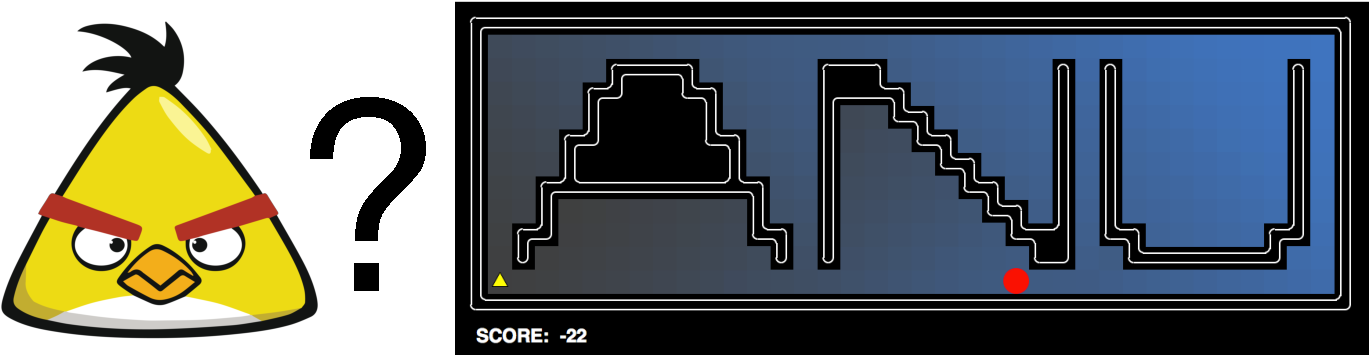
\includegraphics[width=130mm]{WhereIsChuck.pdf}
\end{figure}


\section{Background}

Chuck, the Yellow Bird, is lost in a maze. Time for you to guide Red, the Red Bird, to look for him!\\

Throughout this assignment you will implement some search strategies to help Red find a path to Chuck.
You will write an admissible heuristic to help Red find multiple clones of Chuck in a maze.
You will also write parts of a minimax algorithm to help Red find more Chuck clones than Black, the
black bird.\\

To do this assignment, you mainly need to look at the files \texttt{search\char`_strategies.py},
\texttt{heuristics.py}, and \texttt{minimax\char`_agent.py}. Along with this handout, the comments
in these files should tell you everything that you need to know to get started.


\section{Preliminary: Human Intelligence}

Before you create some AI algorithms to solve the search problems in this assignment,
you can try solving them yourself by using either the arrow keys or \texttt{w}, \texttt{a},
\texttt{s}, and \texttt{d} to move Red around the maze
With the following command:\\

\texttt{./testKeyboard.sh layout}\\

where layout can be any one of:
\begin{itemize}
\item \texttt{aiSearch}, \texttt{anuSearch}, or \texttt{mazeSearch} to help Red find Chuck;
\item  \texttt{aiMultiSearch}, \texttt{anuMultiSearch}, \texttt{trickyMultiSearch}, or
\texttt{mazeMultiSearch} to help Red find all of the Chuck clones; or
\item \texttt{smallAdversarial}, \texttt{testAdversarial}, \texttt{aiAdversarial}, or
    \texttt{anuAdversarial} to help Red find more Chuck clones than Black.
\end{itemize}


\section{Q1: Depth-First Search (2 marks)}

In the \texttt{depth\char`_first\char`_search} function in \texttt{search\char`_strategies.py},
implement the depth-first search algorithm to find Chuck.
You can test your solution with the following commands:\\

\texttt{./testDFS.sh aiSearch}\\
\indent \texttt{./testDFS.sh anuSearch}\\
\indent \texttt{./testDFS.sh mazeSearch}\\

You should see the states explored in your search in a blue hue, 
where the brighter the hue indicates the earlier the exploration.
%For full marks, you need to take care to {\bf avoid expanding} any already-expanded
%states in your implementation.\\

You can implement a generic search function for handling Q1-Q3. However,
this is not necessary for you to receive full marks for the questions.\\

Look in \texttt{frontiers.py} for a \texttt{Stack} (LIFO) data-type that you may find useful
for this exercise.

\section{Q2: Breadth-First Search (2 marks)}

The depth-first search algorithm may not find the shortest path to Chuck, but as
you should have seen from the expanded nodes, it may not have to explore much of the
search space to find a solution.\\

To get the shortest solution, implement the breadth-first search algorithm in
the \texttt{breadth\char`_first\char`_search} function in \texttt{search\char`_strategies.py}. 
To test your implementation, use the following commands:\\

\texttt{./testBFS.sh aiSearch}\\
\indent\texttt{./testBFS.sh anuSearch}\\
\indent\texttt{./testBFS.sh mazeSearch}\\

If you have implemented BFS correctly, Red should find Chuck in 26 steps (with a score of 74) in aiSearch,
45 steps (with a score of 55) in anuSearch, and
68 steps (with a score of 32) in mazeSearch.\\

Look in \texttt{frontiers.py} for a \texttt{Queue} (FIFO) data-type that you may find useful
for this exercise.

\section{Q3: A-Star Search (3 marks)}

Breadth-first search always find the shortest solution, but it can be very costly in
expanding a lot of search nodes. To minimise search cost, a smarter search is needed.\\

A-star search is a smart search if you use the right heuristic.
Implement A-star search in the function \texttt{a\char`_star\char`_search} in \texttt{search\char`_strategies.py}.
You can then test your solution with the Manhattan Distance heuristic (already implemented) with the following commands:\\

\texttt{./testAStar.sh aiSearch manhattan}\\
\indent\texttt{./testAStar.sh anuSearch manhattan}\\
\indent\texttt{./testAStar.sh mazeSearch manhattan}\\

If you have implemented A-star search correctly, you'll find that Red finds Chuck
with the same path length, but with fewer search nodes expanded.\\

You can also try this using Euclidean distance as a heuristic by substituting
\texttt{manhattan} for \texttt{euclidean} in the above examples.\\

Look in \texttt{frontiers.py} for a \texttt{PriorityQueue} data-type that you may find useful
for this exercise. Additionally, there is an optional \texttt{PriorityQueueWithFunction} class
which allows you to pass an evaluation function to make it easier to write a
generic search function for Q1-Q3 if you want to.\\

Once you are finished, you may wish to think of other, stronger heuristics here.
You may notice that it can be quite difficult to think of admissible heuristics which are not
just as expensive to compute as the original problem is to solve!


\section{Q4: Find Every Yellow Bird (4 marks)}
Now there are many Yellow Birds lost in the maze. 
You have to guide Red to find them all!
%
This is a much more difficult problem than finding a single bird.
A solution consists of a path that find every yellow bird.\\

If you have implemented A-star search in the previous question correctly,
you can already solve small problems such as \texttt{testSearch} by typing:\\

\texttt{./testEveryBirdNull.sh aiMultiSearch}\\
\indent\texttt{./testEveryBirdNull.sh anuMultiSearch}\\
\indent\texttt{./testEveryBirdNull.sh smallMultiSearch}\\
\indent\texttt{./testEveryBirdNull.sh mazeMultiSearch}\\

However, you'll find that it can be very slow for some problems, such as \texttt{mazeMultiSearch}.
To solve this last problem with the null heuristic, A-star has to expand over $500000$ nodes!
%
To optimise your search, you need to build your own heuristic to find every yellow bird in the maze.
Implement \texttt{every\char`_bird\char`_heuristic} with an {\bf admissible heuristic} in \texttt{heuristics.py}.
You can test your heuristic with the following commands:\\

\texttt{./testEveryBird.sh aiMultiSearch}\\
\indent\texttt{./testEveryBird.sh anuMultiSearch}\\
\indent\texttt{./testEveryBird.sh smallMultiSearch}\\
\indent\texttt{./testEveryBird.sh mazeMultiSearch}\\

You will be graded on how many nodes your search expanded on the \texttt{smallMultiSearch} map.
The fewer search nodes explored, the more points you'll get:

\begin{itemize}
\item $> 15000$ nodes: 1/4
\item $\leq 15000$ nodes: 2/4
\item $\leq 8000$ nodes: 3/4
\item $\leq 7000$ nodes: 4/4
\end{itemize}

If you can solve \texttt{smallMultiSearch} and \texttt{mazeMultiSearch}, expanding less than $2000$ nodes
in less than $30$ seconds (on our test machine) with an admissible heuristic then you will be awarded
one bonus point to make up for marks if you lose them elsewhere in the assignment.
We have a solution to this problem which expands $698$ nodes and takes $0.8$ seconds.\\

You need to explain in the comments of your heuristic why it is admissible.
You will suffer a two point penalty to the mark awarded to your heuristic if it is not admissible, so
be careful!\\

The comments in \texttt{every\char`_bird\char`_heuristic} detail the data structures you
will need to use. In particular, we have gone to the trouble of pre-computing
the shortest distance between every pair of positions on every map.
As described in the comments this information is available to you using the
\texttt{maze\char`_distance} function.

\section{Q5: Minimax (4 marks)}

Now Bomb, the black bird and Red are having a race to see who can find the most lost yellow birds.\\

Bomb really wants to help as many yellow birds as possible and greedily runs towards the
closest yellow bird to him at any time. He will only stand still if there is nowhere he can move.
To see how he behaves, look at the class \texttt{GreedyBlackBirdAgent} at the
bottom of \texttt{agents.py}.
To help Red win the race we are going to use the {\em Minimax algorithm}.\\

In this setting the utility of a terminal state is the score of that state as displayed in
the user interface. 
%Red scores $100$ points for every yellow bird he saves and loses
%$100$ points for every yellow bird Bomb saves. 
Red scores a number of points for every yellow bird he saves and loses
points for every yellow bird Bomb saves. The yellow birds are
initially worth $100$ points, but the value of each unsaved yellow
bird decreases by 1 at every move (this helps giving Red and Bomb a
sense of urgency!).  Red has to get a positive score to win. Red wants
to have the highest score overall, even if he ends up losing.\\
%Red has to save more yellow birds than Black to win. 

Implement the required methods in \texttt{MinimaxAgent} in \texttt{minimax\char`_agent.py}.
First, you will need to implement the methods \texttt{maximize} and \texttt{minimize}.\\

You can then test your implementation with:\\

\texttt{./testMinimax.sh testAdversarial depth}\\
\indent\texttt{./testMinimax.sh smallAdversarial depth}\\
\indent\texttt{./testMinimax.sh aiAdversarial depth}\\
\indent\texttt{./testMinimax.sh anuAdversarial depth}\\

Here, \texttt{depth} is the maximal depth of the game tree explored.
In your implementation
each maximization or minimization should count as one depth step.\\

You should notice that it is too computationally expensive to set the depth high enough to explore
the whole search space. When the depth limit is reached the algorithm calls
\texttt{simple\char`_evaluation} instead of \texttt{utility}. This evaluation represents
an estimate of the utility.\\

The implementation of \texttt{evaluation} we have provided the search just returns
the utility of the reached state, rather than the expected utility at the end of the game.
You need to implement your own, more powerful evaluation in this method.\\

You should hopefully be able to perform competitively with the Black Bird on these maps
with a depth of $10-12$.\\

You will be awarded $2$ of the $4$ points for this exercise for the correctness of your
\texttt{minimize} and \texttt{maximize} methods and a further $2$ points for the
quality of your \texttt{advanced\char`_evaluation} method.


%\section{Q6: AlphaBeta Pruning (4 marks)}
%
%Minimax can be made more efficient with AlphaBeta Pruning, which reduces the number of search state explored without affecting correctness. A variant of this algorithm was implemented in the DeepBlue chess computer which beat world champion Garry Kasparov.
%
%Implement \texttt{AlphaBetaAgent} in \texttt{adversarialSearchAgents.py}. Similar to MinimaxAgent in the previous question, your implementation should handle multiple Black Birds, and its minimax value should be identical to that of MinimaxAgent. Again, the correctness of your implementation will be checked with the correct number of states expanded. This can be tested with the following command:\\
%\\
%\texttt{./testAlphaBeta.sh}\\
%\\
%Similar to \texttt{Minimax}, Red may run into a Black Bird in some cases. This is to be expected. 

\section{Submission}

When you have finished the assignment, make and submit (on Wattle) a \texttt{uxxxxxx.tgz} file containing 
the following files:\\
\\
\texttt{search\char`_strategies.py}\\
\texttt{heuristics.py}\\
\texttt{minimax\char`_agent.py}\\

Auto-grading will be used to assess the correctness of your code, but all submissions
will be looked at manually as well. Please comment your code as it helps us to
determine your intent and give part marks when things don't work as intended.

\bibliographystyle{abbrv}

%\begin{thebibliography}{}
%
%\bibitem{smh} 
%J. Robertson.
%{\em In the wild world of Angry Birds, man triumphs over machine},
%The Sydney Morning Herald, 07.12.2012. 
%\url{http://www.smh.com.au/digital-life/games/in-the-wild-world-of-angry-birds-man-triumphs-over-machine-20121206-2ay9c.html}
%
%\end{thebibliography}

\end{document}
